\begin{frame}
  \begin{center}
    \Huge Problem definition
  \end{center}
\end{frame}

\begin{frame}
  \frametitle{Problem definition}
  Let
  \begin{itemize}
    \item \blue{$D(V = \{s\} \cup V^{+} \cup \{t\}, A)$} be the digraph, where
    \begin{itemize}
      \item \blue{$s$} is the source node; and 
      \item \blue{$t$} is the target node.
    \end{itemize}
    \item \blue{$c_a \in \mathbb{R}$} be the arc \blue{$a \in A$} cost;
    \item \blue{$R$} be the set fo resources;
    \item \blue{$d^r_a \in \mathbb{R}$} be the arc \blue{$a \in A$}' metric resource \blue{$r \in R$} consumption;
    \item \blue{$w^r_i = [b^r_i, e^r_i]$} be the node \blue{$i \in V$}' resource \blue{$r \in R$} window.
  \end{itemize}
  The ERCSPP consists in finding the shortest \blue{$s$}-\blue{$t$}-path in \blue{$D$}.
\end{frame}

\begin{frame}
  \frametitle{Problem definition}
  \blue{$c_a: (d^1_a, d^2_a)$}\\
  \blue{$w_s^1 = w_s^2 = [0,0], w_2^1 = [2, 3], w_2^2 = [0, 1], w_3^1 = [1, 5], w_3^2 = [1, 3], w_t^1 = [3, 5], w_t^2 = [0, 2]$}
  \begin{figure}[H]
    \centering
    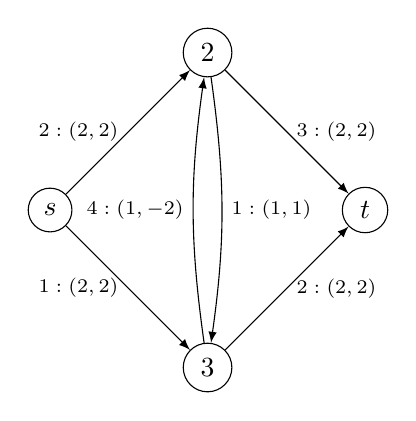
\begin{tikzpicture}
      %nodes
      \node[circle, draw] (s) at (0, 0) {\blue{$s$}};
      \node[circle, draw] (a) at (2, 2) {\blue{$2$}};
      \node[circle, draw] (b) at (2, -2) {\blue{$3$}};
      \node[circle, draw] (t) at (4, 0) {\blue{$t$}};
      %edges
      \path [draw,-latex] (s) to node[left]{\scriptsize\blue{$2: (2, 2)$}} (a);
      \path [draw,-latex] (s) to node[left]{\scriptsize\blue{$1: (2, 2)$}} (b);
      \path [draw,-latex] (a) to node[right]{\scriptsize\blue{$3: (2, 2)$}} (t);
      \path [draw,-latex] (b) to node[right]{\scriptsize\blue{$2: (2, 2)$}} (t);
      \path [draw,-latex] (a) edge [bend left=8] node[right]{\scriptsize\blue{$1: (1, 1)$}} (b);
      \path [draw,-latex] (b) edge [bend left=8] node[left]{\scriptsize\blue{$4: (1, -2)$}} (a);
    \end{tikzpicture}
    \caption{A ERCSPP instance digraph example.}
    \label{fig:vrptw_disposable_example}
  \end{figure}
\end{frame}

\begin{frame}
  \frametitle{Problem definition}
  \blue{$c_a: (d^1_a, d^2_a)$}\\
  \blue{$w_s^1 = w_s^2 = [0,0], w_2^1 = [2, 3], w_2^2 = [0, 1], w_3^1 = [1, 5], w_3^2 = [1, 3], w_t^1 = [3, 5], w_t^2 = [0, 2]$}
  \begin{figure}[H]
    \centering
    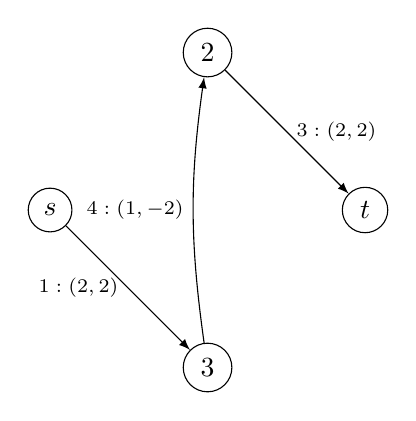
\begin{tikzpicture}
      %nodes
      \node[circle, draw] (s) at (0, 0) {\blue{$s$}};
      \node[circle, draw] (a) at (2, 2) {\blue{$2$}};
      \node[circle, draw] (b) at (2, -2) {\blue{$3$}};
      \node[circle, draw] (t) at (4, 0) {\blue{$t$}};
      %edges
      \path [draw,-latex] (s) to node[left]{\scriptsize\blue{$1: (2, 2)$}} (b);
      \path [draw,-latex] (b) edge [bend left=8] node[left]{\scriptsize\blue{$4: (1, -2)$}} (a);
      \path [draw,-latex] (a) to node[right]{\scriptsize\blue{$3: (2, 2)$}} (t);
    \end{tikzpicture}
    \caption{A ERCSPP instance digraph example.}
    \label{fig:vrptw_disposable_example}
  \end{figure}
\end{frame}
